\documentclass[10pt, a4paper]{exam}
\usepackage{graphicx}
\usepackage[a4paper, total={7in, 9.5in}]{geometry}
\usepackage[normalem]{ulem}
\usepackage{amsmath}
\renewcommand\ULthickness{1.0pt}   
\setlength\ULdepth{1.3ex}

\begin{document}


	\noindent
	\begin{minipage}[l]{0.1\textwidth}
		\noindent
		
\includegraphics[width=2.8\textwidth]{ESCUDO.png}
	\end{minipage}
\hfill
\begin{minipage}[c]{0.8\textwidth}
	\begin{center}
		{\large  Departamento de Ingeniería civil y Agrícola\par
		\large	Facultad de Ingeniería	\par
	% \large \textbf{Taller propiedades de los fluidos}	\par
    \large \textbf{Taller Final}	\par
    Prof. Luis Alejandro Morales Mar\'in, Ph.D. \par
} %%%%% NOMBRE DEL PROFESOR 
	\end{center}
\end{minipage}
\par
\vspace{0.2in}
\noindent
    \uline{Estructuras hidráulicas [2015954]	\hfill 2025-I}
\par 
\vspace{0.15in}
\noindent

%%%%%%%%%%%%%%%%%%%%%%%%%%%%%



\begin{enumerate}

    \item Considérese la sección transversal del colector representada en la figura~\ref{fig:colector}. La pendiente longitudinal de colector es 0.0004 y el coeficiente de Manning es 0.014. Determínese el caudal circulante (en régimen permanente y uniforme) para la profundidad máxima del flujo representada si el canal de caudales bajos es de geometría semicircular.
    \begin{figure}[h!]
        \centering
        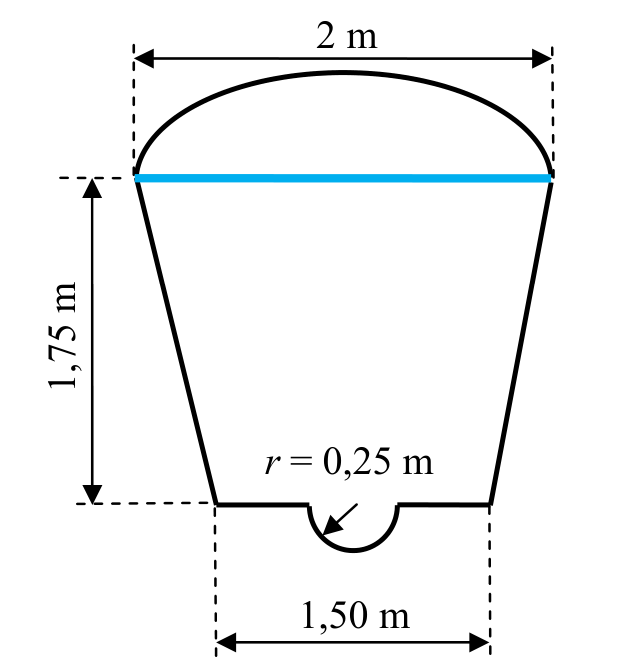
\includegraphics[width=0.3\linewidth]{Images/colector.png}
        \caption{Representación del colector.}
        \label{fig:colector}
    \end{figure}

    \item Calcúlese el caudal circulante en la sección del cauce de la figura~\ref{fig:trapcompus} para flujo en régimen permanente y uniforme si la pendiente longitudinal es del 2\% y el coeficiente de Manning es igual a 0.045.
    \begin{figure}[h!]
        \centering
        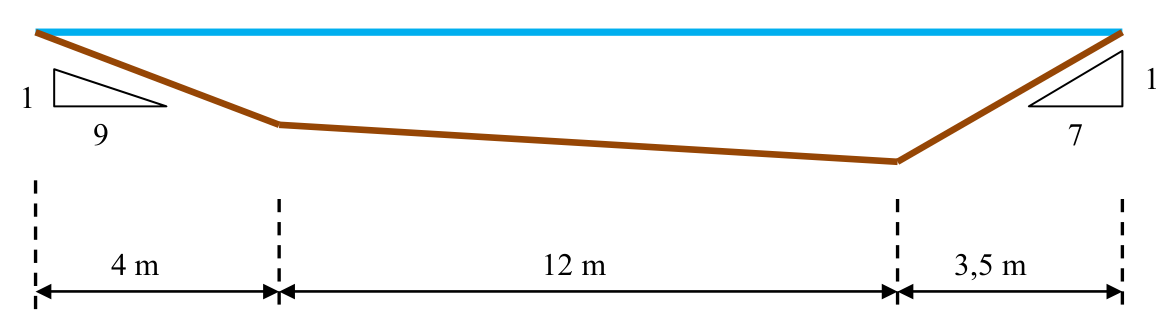
\includegraphics[width=0.6\linewidth]{Images/trapcompus.png}
        \caption{Sección del cause.}
        \label{fig:trapcompus}
    \end{figure}

    \item Sea un canal de laboratorio de pendiente variable (entre el 0.001\% y el 2\%) cuya sección es triangular simétrica (véase la figura \ref{fig:triangulo}). Supóngase un tramo intermedio del canal en el que el flujo circula en régimen permanente y uniforme. Determínese el valor de la energía específica mínima en el canal para dicho tramo e intervalo de pendiente, si el caudal se mantiene constante a $0.4m^3/s$.
    \begin{figure}[h!]
        \centering
        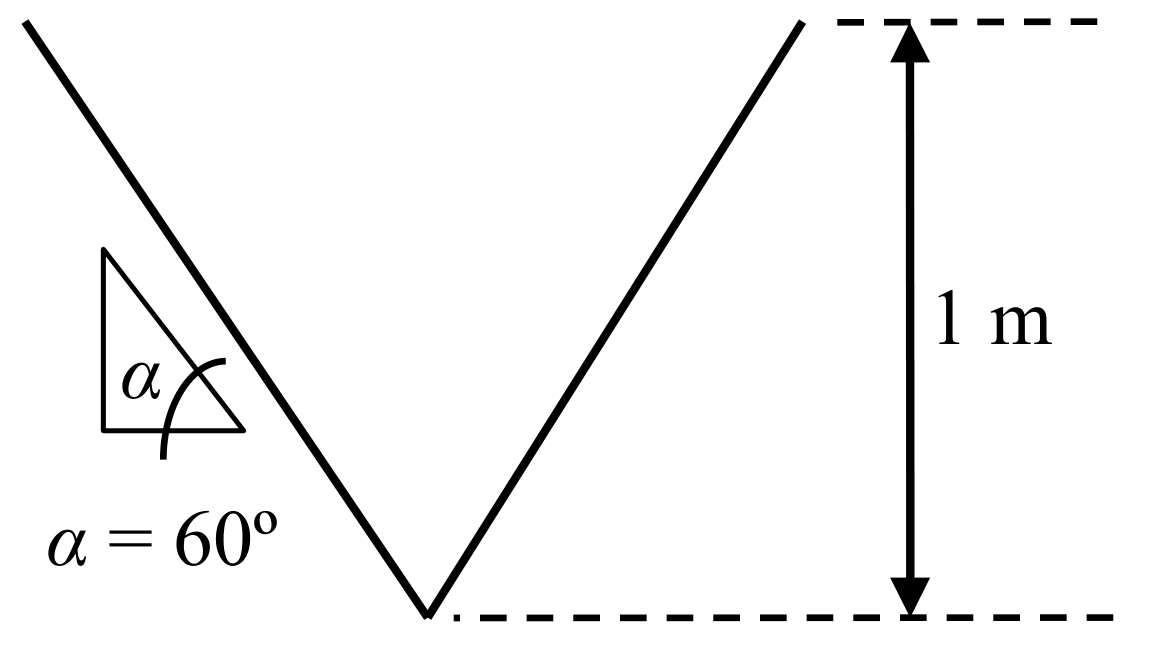
\includegraphics[width=0.35\linewidth]{Images/triang.png}
        \caption{Sección triangular.}
        \label{fig:triangulo}
    \end{figure}

    \item Un depósito alimenta a un canal trapezoidal de ancho de $1m$, talud $Z=1$, coeficiente de rugosidad $0.014$ y pendiente $0.0005$. A la entrada, la profundidad de agua en el depósito es de $0.736 m$ por encima del fondo del canal como se muestra en la figura \ref{deposit}. Determinar el caudal en el canal con flujo uniforme subcrítico, suponiendo que la pérdida a la entrada es $0.25 \cdot v^2_1/2g$.
    \begin{figure}[h!]
        \centering
        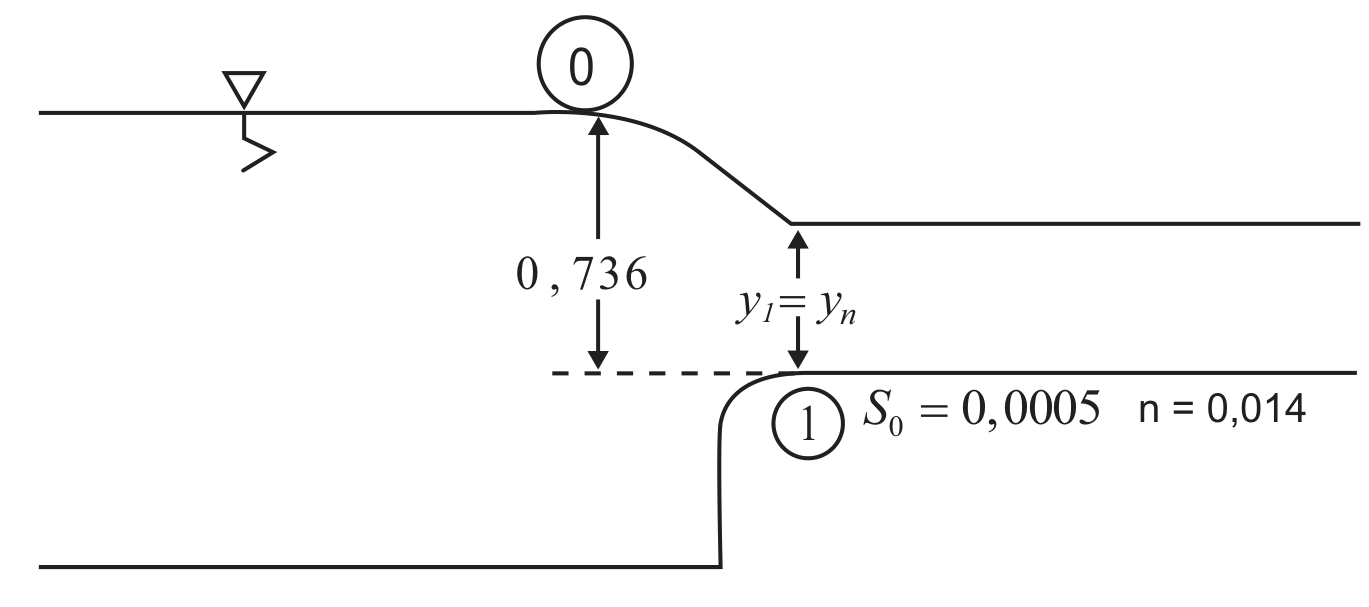
\includegraphics[width=0.5\linewidth]{Images/deposit.png}
        \caption{Perfil longitudinal del depósito y canal.}
        \label{deposit}
    \end{figure}    

    \item Sea un canal prismático de sección rectangular de $4 \ \mathrm{m}$ de ancho y coeficiente de Manning de $0.016$, por el que circulan $71 \ \mathrm{m}^3 \cdot \mathrm{s}^{-1}$.

    En función de la pendiente se distinguen dos tramos. Uno, aguas arriba, de longitud ilimitada y cuya profundidad normal es de $1.20 \ \mathrm{m}$. Otro, aguas abajo, construido en un Box-Culvert de $2 \ \mathrm{m}$ de altura, con pendiente del $1\%$, de $200 \ \mathrm{m}$ de longitud y que finaliza en una caída vertical (véase la figura \ref{fig:7}).

    Para las citadas condiciones:

    \begin{itemize}
        \item[(a)] Dibújese de forma aproximada el perfil longitudinal de la lámina libre del agua en los dos tramos, indicando el tipo de perfil.
        \item[(b)] Compruébese si el flujo circula en lámina libre a lo largo de todo el recorrido del Box-Culvert.
    \end{itemize}

    \begin{figure}[h!]
        \centering
        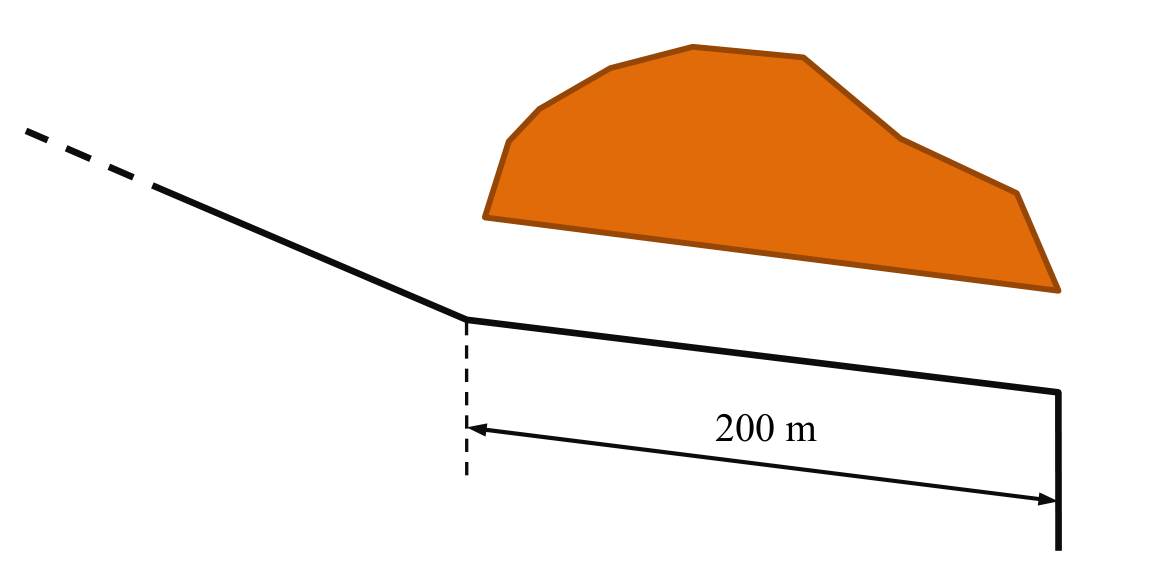
\includegraphics[width=0.5\linewidth]{Images/7.png}
        \caption{Condiciones del canal con Box-Culvert.}
        \label{fig:7}
    \end{figure}

    \item Sea un cauce de sección rectangular de $14 \ \mathrm{m}$ de ancho y $n = 0.020$, por el que circulan $50 \ \mathrm{m}^3 \cdot \mathrm{s}^{-1}$.

    Se distinguen dos tramos en función de la pendiente longitudinal. Uno, situado aguas arriba y de longitud indefinida, cuya pendiente es $5 \cdot 10^{-4} \ (\mathrm{m} \cdot \mathrm{m}^{-1})$, y otro, aguas abajo, de $30 \ \mathrm{m}$ de longitud que finaliza en una caída vertical y cuya pendiente es del $1\%$.

    A $15 \ \mathrm{m}$ aguas arriba de la sección de caída se halla una compuerta con desagüe de fondo cuya abertura es de $90 \ \mathrm{cm}$ (véase la figura \ref{fig:9}).

    Compruébese si en las condiciones descritas la compuerta influye en el flujo.

    \begin{figure}[h!]
        \centering
        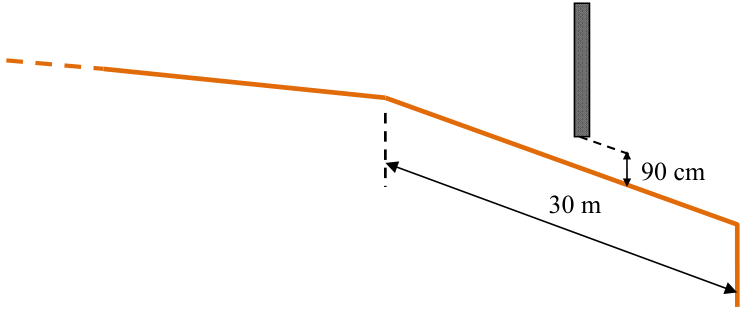
\includegraphics[width=0.47\linewidth]{Images/9.png}
        \caption{Condiciones del canal con compuerta.}
        \label{fig:9}
    \end{figure}

\item A series of tests have been conducted to a vee weir of $90^\circ$. Determine the discharge coefficient ($C_d$) based on the data in table~\ref{tab:1}.

    \begin{table}[h!]
    \centering
    \begin{tabular}{|c|c|c|c|c|c|c|c|c|}
    \hline
    $h_1$ (m) & 0.201 & 0.205 & 0.195 & 0.210 & 0.204 & 0.196 & 0.198 & 0.200 \\
    \hline
    $Q$ (L/s) & 25.1  & 25.4  & 25.0  & 25.6  & 25.5  & 24.9  & 24.9  & 25.1  \\
    \hline
    \end{tabular}
    \caption{Measured data for vee weir tests.}
    \label{tab:1}
\end{table}

\item Sobre una placa con las dimensiones que se presentan en la figura~\ref{fig:21} se produce un vertido superior y una descarga por el orificio del fondo. El ancho de la placa es de $1.00 \ \mathrm{m}$ y es igual al del canal.

    Determinar cuál es el gasto de vertido si el del orificio es $Q_o = 0.3 \ \mathrm{m}^3/\mathrm{s}$, suponiendo que en ambos la descarga es libre. Asuma un $C_d=0.595$  

    \begin{figure}[h!]
        \centering
        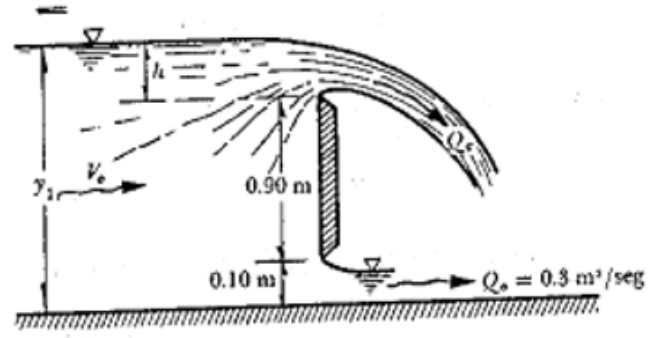
\includegraphics[width=0.4\linewidth]{Images/21.png}
        \caption{Configuración del vertedero y el orificio.}
        \label{fig:21}
    \end{figure}

 \item Por un canal rectangular de ancho $2.0 \ \mathrm{m}$ circula agua con caudales entre $Q_\mathrm{min} = 20 \ \mathrm{l/s}$ y $Q_\mathrm{max} = 600 \ \mathrm{l/s}$.
    
    Este caudal se debe medir usando:
    
    \begin{itemize}
        \item Un vertedero rectangular de pared delgada (sin contracción)
        \item Un vertedero triangular de pared delgada con una abertura de $90^\circ$
        \item Un vertedero de pared gruesa
    \end{itemize}
    
    En todos los casos $P = 1.0 \ \mathrm{m}$. Hacer una gráfica de $H$ (vertical) vs $Q$ (horizontal) para cada vertedero e indique cuál vertedero sería el mejor para esta aplicación.

\item  Sea un canal revestido de hormigón ($n = 0.011$) de sección trapecial simétrica de $7 \ \mathrm{m}$ de base e inclinación de los márgenes $1.5 \ \mathrm{H} : 1.0 \ \mathrm{V}$, cuya pendiente longitudinal es del $5\%$.

    Dicho canal une una balsa y una caída vertical que se encuentran separados $100 \ \mathrm{m}$ (véase la figura \ref{fig:3}). El nivel de la lámina de agua en la balsa se considera constante, siendo $1.54 \ \mathrm{m}$ la diferencia de cota entre la lámina de agua en la balsa y el lecho al inicio del canal. Determínese la profundidad en la sección de caída y el perfil de la lámina de agua con incrementos en la profundidad de $5 \ \mathrm{cm}$.

    \begin{figure}[h]
        \centering
        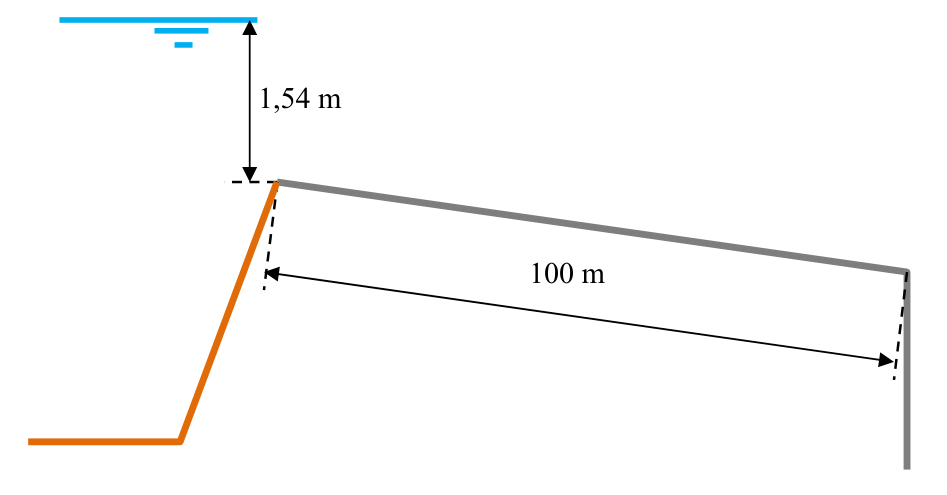
\includegraphics[width=0.5\linewidth]{Images/3.png}
        \caption{Condiciones y configuración iniciales del canal.}
        \label{fig:3}
    \end{figure}

\end{enumerate}

    
\end{document}



